% \documentclass{article}
\documentclass[12pt, letterpaper]{article}  % it must be at least 11 pt or more if you like (here we used 12 for clarity of the demo), and change article with report
% \usepackage[letterpaper, top=3.71cm, bottom=3.20cm, left=2.86cm, right=2.86cm]{geometry}

\usepackage [a4paper, top=1.5cm, bottom=1.25cm, left=2cm, right=2cm]{geometry}

\usepackage[utf8]{inputenc}
\usepackage{placeins}
\usepackage{booktabs}
\usepackage{array}
% \usepackage{caption}
\usepackage{subfig}
\usepackage{hyperref}
\usepackage{graphicx}
\usepackage{biblatex} %Imports biblatex package
\usepackage[english]{babel}
\usepackage[utf8]{inputenc}
% \usepackage[T1]{fontenc}
\usepackage{xcolor}
\usepackage{listings}
\usepackage{amsmath}
\usepackage{float}
\usepackage{siunitx}
\usepackage{url}
\usepackage{dirtree}
% \usepackage{geometry}
% \geometry{a4paper, top=1.5cm, bottom=1.25cm, left=2cm, right=2cm}


\title{\textit{Huffman Encoding}}
\author{Anas Shamoon}
\date{September, 2023}

\begin{document}
\begin{titlepage}
	\maketitle
	\pagenumbering{gobble}
   \begin{center}
	\vspace{0.5cm}
       Final project for the\\ \textit{Parallel and Distributed Systems: Paradigms and Models}\\ course
       \vfill	     
       
\includegraphics[width=0.2\textwidth]{Images/unipi.png}\\
       University of Pisa\\
       A.Y. 2022/2023\\
   \end{center}
\end{titlepage}
\newpage

\setcounter{tocdepth}{7}
\setcounter{secnumdepth}{4}

\maketitle

\begin{center}
\hspace{0.5cm}
{\footnotesize \tableofcontents}
\end{center}

\pagenumbering{arabic}

\newpage

\section{Introduction}
This report contains the design and implementation choices for the Huffman Encoding project. The timing of the sequential algorithm will first be shown, and then the chosen parallel design will be described, giving reasons for the choices. Finally, speedup, scalability and efficiency results will be illustrated. 
\section{Sequential Algorithm}
Before parallelizing the program, it's necessary to know how the sequential code works and what part of the part can be parallelized (the generic stages of the sequential program is shown in figure \ref{fig:seq_code}).
\begin{figure}[h!]
    \centering
    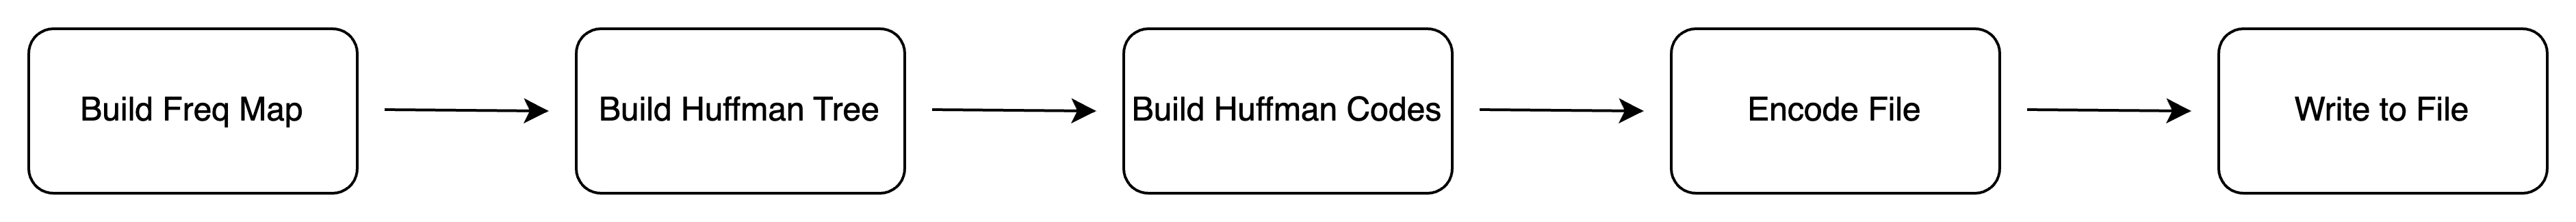
\includegraphics[width=1 \textwidth]{Images/sequential-stages.png}
    \caption{Sequential Algorithm Stages}
    \label{fig:seq_code}
\end{figure}
\FloatBarrier

The computation times have been estimated using a 556 MBs input text file.

\begin{center}
\begin{tabular}{ |c|c| }
 \hline
 \textbf{Stages}& \textbf{Time (usec)} \\
 \hline
 Frequency Map & 14838749 \\
 \hline
 Huffman Tree & 10 \\
 \hline
 Huffman Codes & 10 \\
 \hline
 File Encoding & 20041386 \\
 \hline
 File Writing & 23068124 \\  
 \hline
\end{tabular}
\end{center}
\FloatBarrier

After analysing the times of the sequential algorithm, the next step was to assess a potential parallel pattern, taking into account that the most computationally intensive aspects of the program which are creating the frequency map, file encoding and file writing.

\section{Parallel Design}
First of all, it was considered appropriate to parallelize the $File Encoding$ phase. In this case, map pattern was adopted which returns the encoded text for the file chunks. The load balancing on the worker threads was taken care of. The file content was divided into equal number of chunks (each worker thread had a start and end pointer to read from the file) and then encoded using the sequentially built Huffman codes. \\
The other alternative approach considered was of having pipeline pattern. It was later on rejected on the fact that pipeline is useful to improve the overall throughput of the system for the streams and our goal in this case of Huffman encoding was to reduce the time taken while encoding the file by reducing the overall latency. The pipeline implementation would have waited for each chunk of file to get processed one by one and when one chunk of the file has been encoded, then it would have moved to the next chunk. \\

Figure \ref{fig:map_pattern} shows the algorithm stages after parallelization.

\begin{figure}[h!]
    \centering
    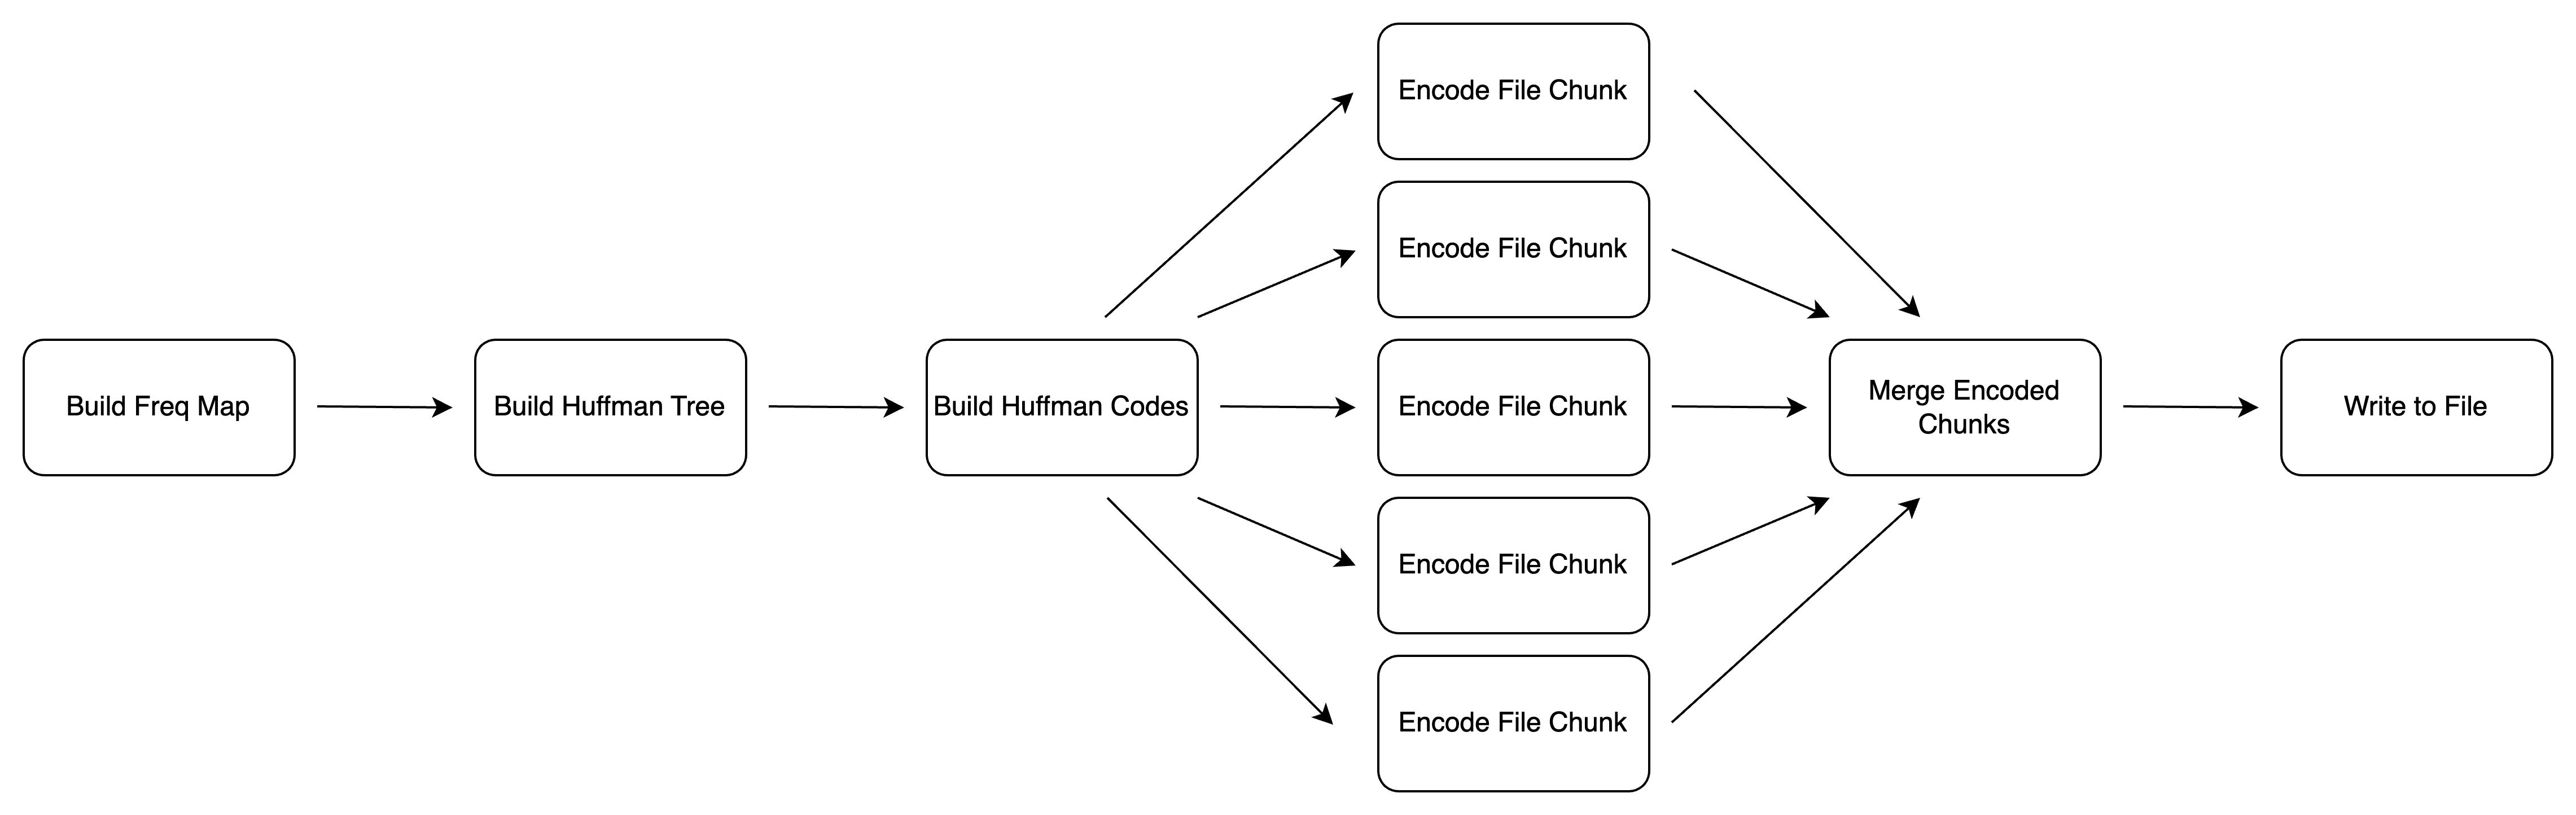
\includegraphics[width=1 \textwidth]{Images/map-pattern.png}
    \caption{Algorithm after parallelization}
    \label{fig:map_pattern}
\end{figure}
\FloatBarrier

\subsection{Native Threads C++}
The initial implementation for parallelization was developed using the native threads in C++. \\

The encoding of the file chunks was achieved by map pattern using the native threads in C++. The overhead in this case was associated with the threads creation and joining. \\

As described in Figure \ref{fig:map_pattern}, the frequency map, Huffman tree and Huffman codes were computed sequentially and then the task of encoding the file was parallelized. The file was divided into equal chunks (start and end pointer for reading file were passed) and each worker thread read the chunk of file and encoded it using the Huffman codes generated in the earlier step. Once all the worker threads are finished with encoding their respective chunks of file, these encoded chunks are then merged into global encoded content which was then written to the file.

\subsection{FastFlow}
The second implementation of the project was developed using the FastFlow library, a programming framework specifically designed for parallel programming in C++. The parallel design remains the same in the second implementation, and it is achieved using ``ff\_farm" class with only the workers. \\

A farm of worker threads equal to number of threads supplied from the command line are created (implemented as ``ff\_node") and the encoding of the file is done in chunks in each worker thread. Once the worker threads are instantiated, the farm is then run and the main thread waits till all the worker nodes complete their computation. Once the computation is completed, the encoded chunks are then merged into global encoded content and then written to the output file.

\section{Results}

The final phase of the project involved performance analysis of the parallel programs, focusing on speedup and scalability. The input file files of various sizes were tested ranging from 1.2MBs till 556 MBs files. Final results are all based on the input text file of size 556 MBs. \\

The programs (sequential, native threads, Fastflow) were ran multiple times to have average times. The parallel programs were ran for threads starting from 1 till 64. \\

In general, there is a significant difference between the ideal and actual execution times in both parallel versions of the program. In the parallelized version of the program, the overhead is mainly due to two main reasons.
\begin{itemize}
    \item Thread creation and joining.
    \item The chunk of the program that has been parallelized due to a fact that the time taken by the chunk of code to read file in threads and encoding file do not differ that much when increasing the number of threads after a certain number of threads. The time reduces significantly for a fewer number of threads than having more number of threads and this can be verified from the graphs below too.
\end{itemize}

In general, both in the case of native threads and FastFlow, the difference between the achieved speedup and the ideal speedup tends to decrease as the number of threads increases (same goes for the scalability and efficiency too).

\subsection{Speedup Plots}
\begin{figure}[H]
\centering
    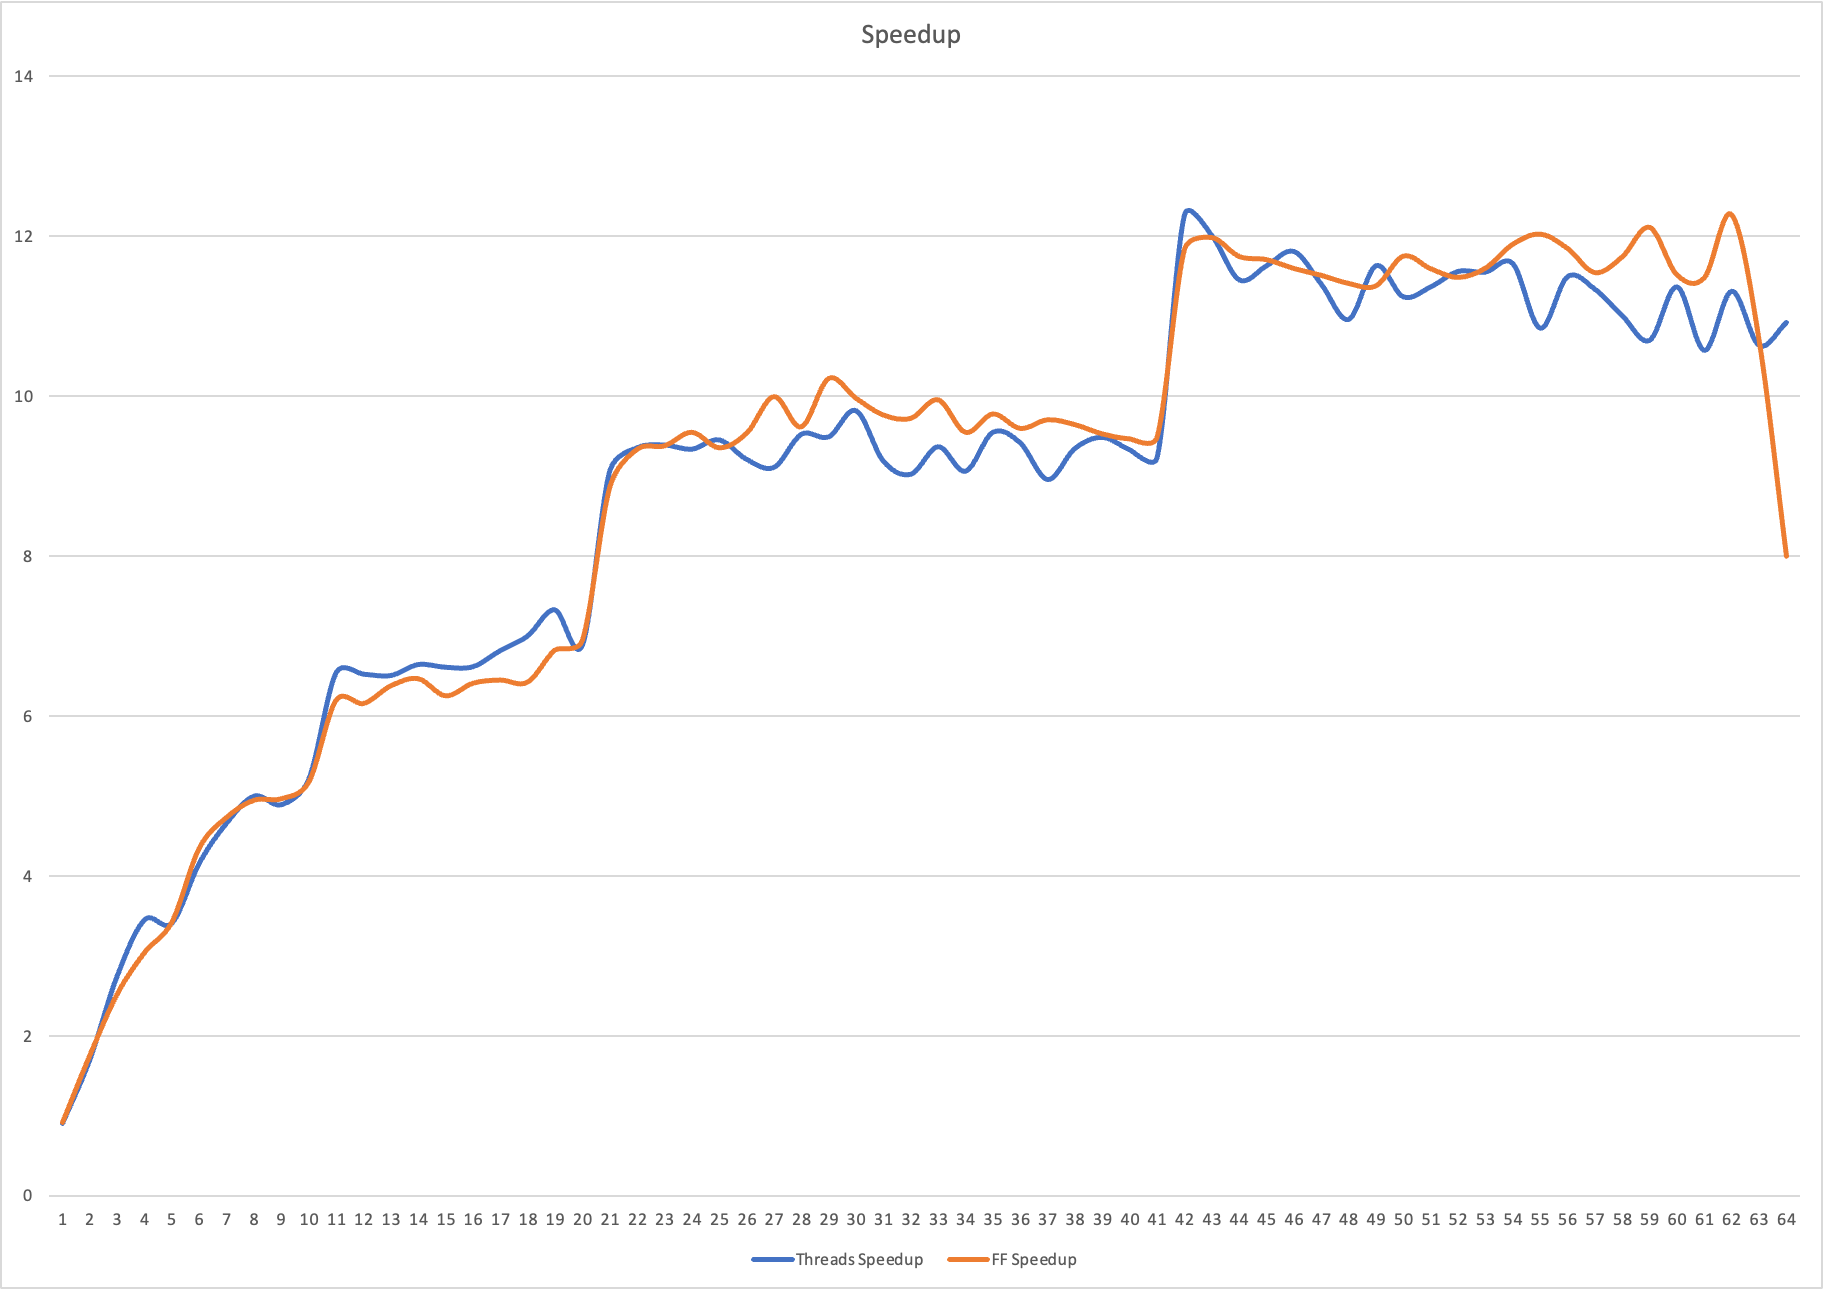
\includegraphics[width=1 \textwidth]{Images/speedup.png}
    \caption{Speedup}
\end{figure}

\textbf{Note:} Maximum speedup of approx 13 is achieved with 43 threads.

\subsection{Scalability Plots}
\begin{figure}[H]
\centering
    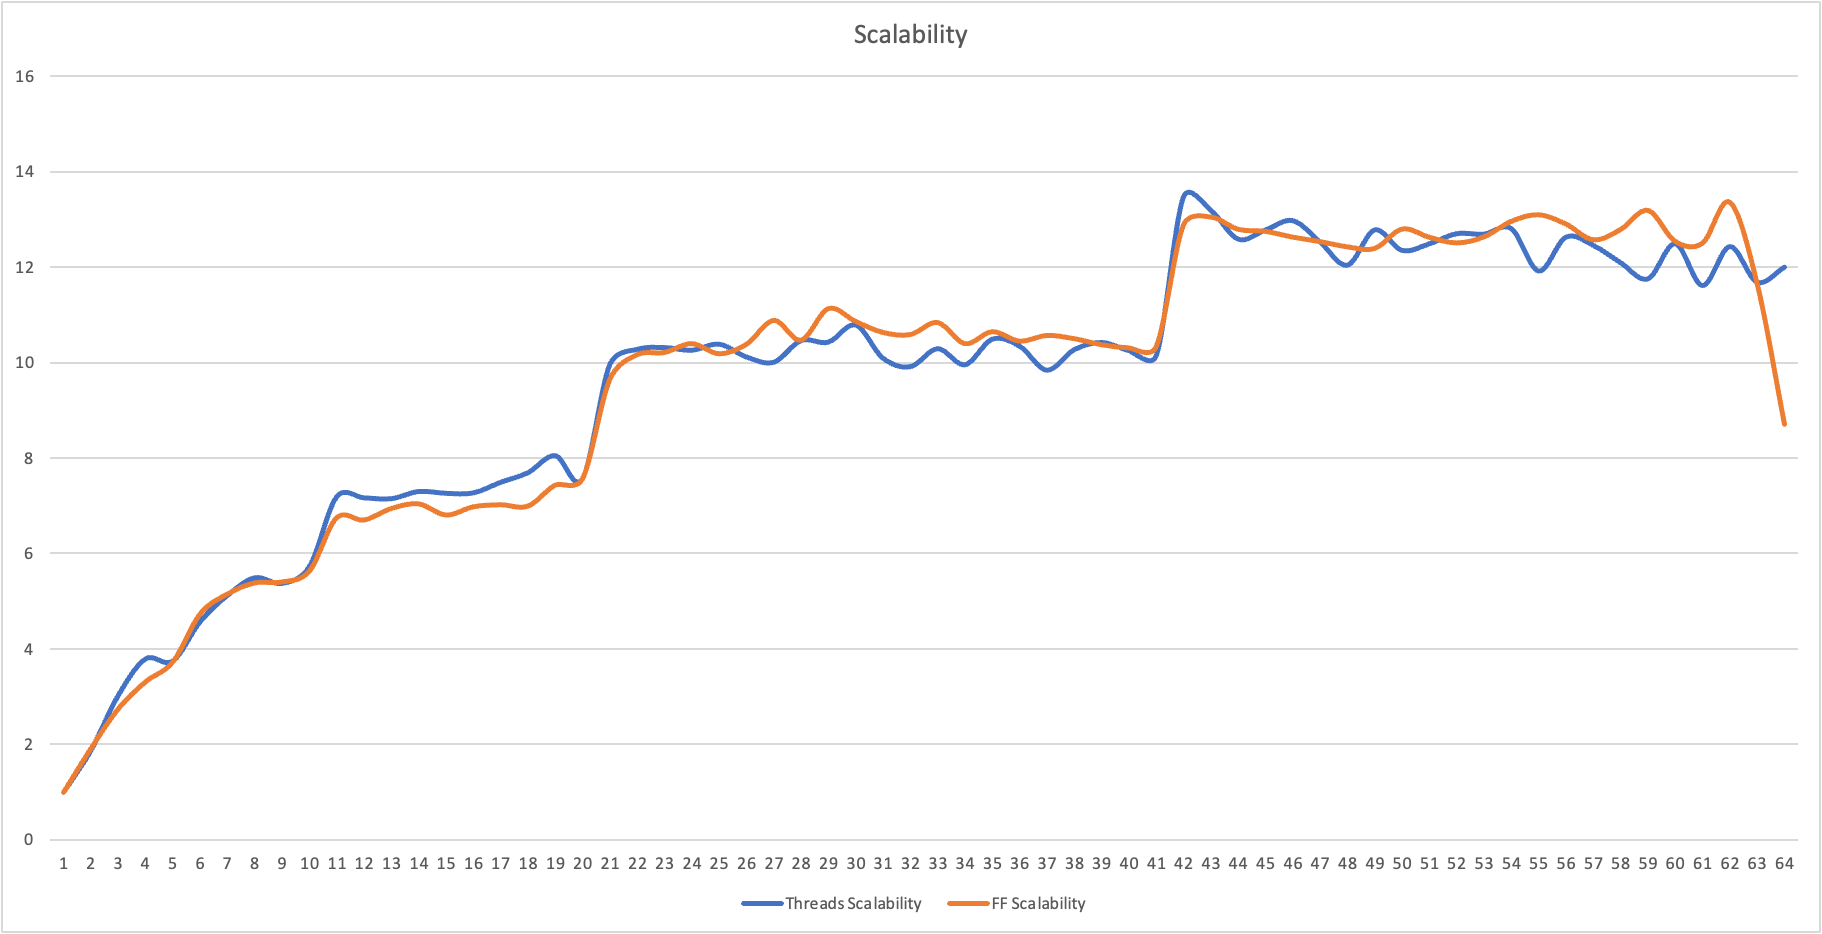
\includegraphics[width=1 \textwidth]{Images/scalability.png}
    \caption{Scalability}
\end{figure}

\textbf{Note:} Maximum scalability of approx 13 is achieved with 43 threads.

\subsection{Efficiency Plots}
\begin{figure}[H]
\centering
    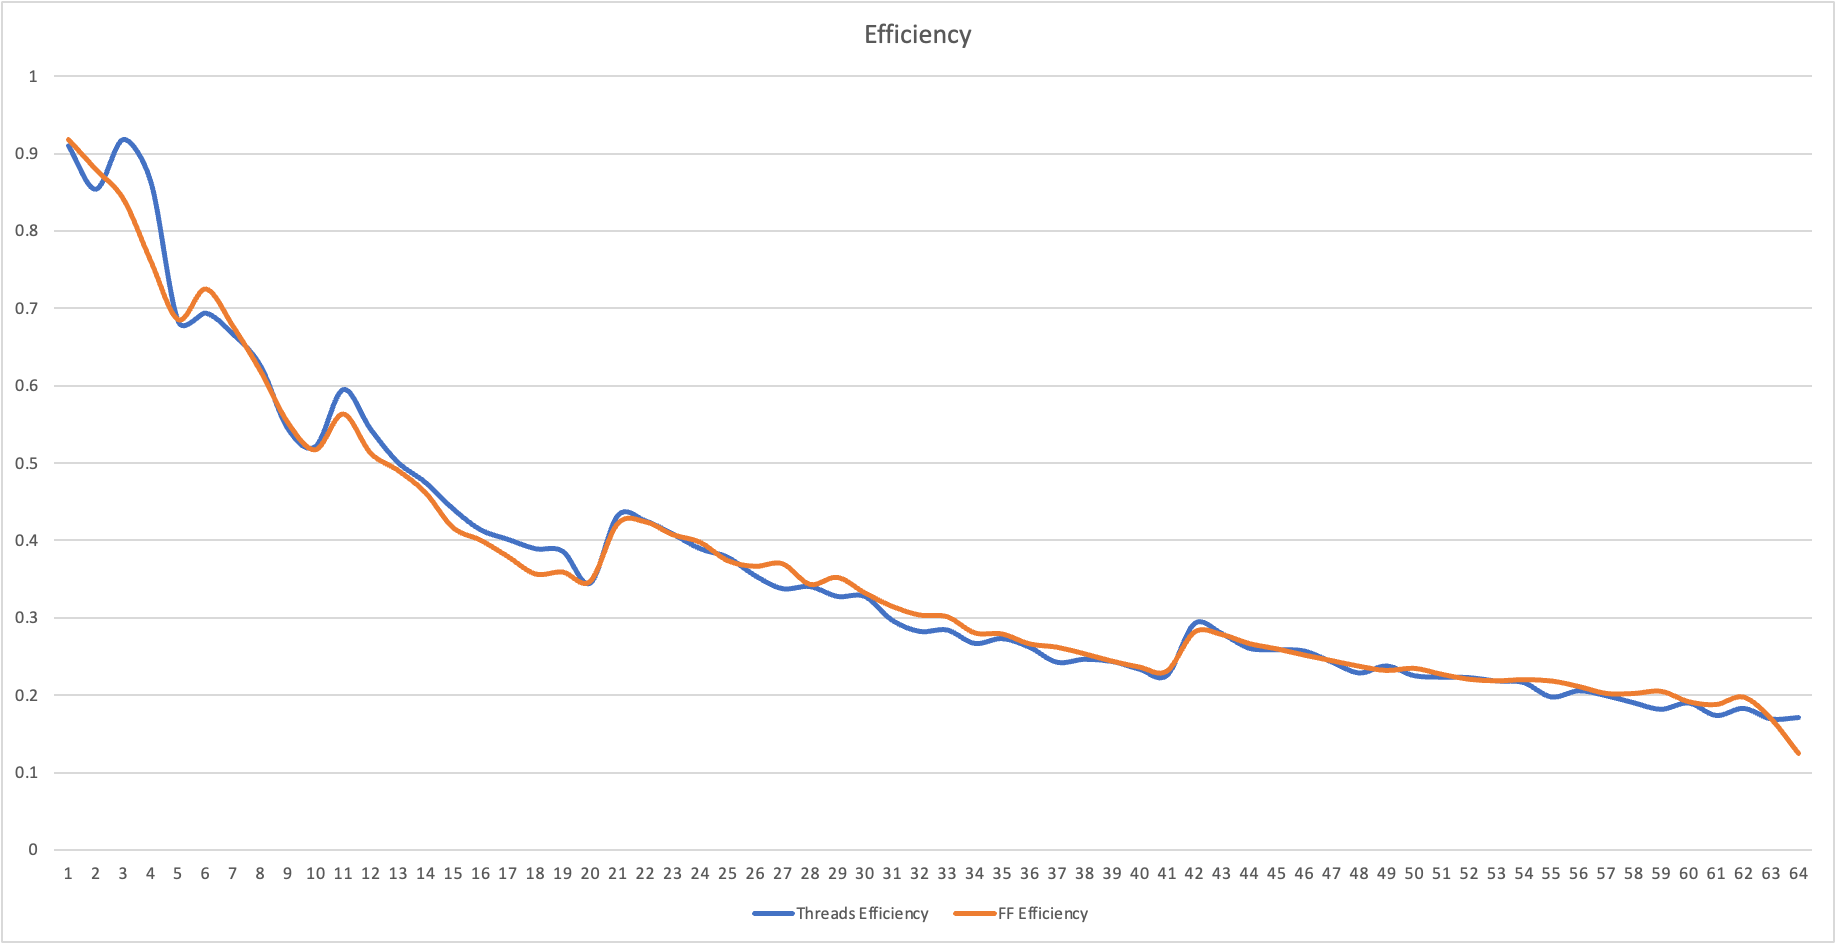
\includegraphics[width=1 \textwidth]{Images/efficiency.png}
    \caption{Efficiency}
\end{figure}

\textbf{Note:} Both the native threads implementation and the Fastflow implementation had similar performance and are below the ideal behavior of linear behavior for speedup and scalability and a constant 1 in case of efficiency.

\section{How to Compile}

The directory structure should be as follows:
\dirtree{%
.1 project.
.2 inputs.
.3 essay\_1.txt.
.2 outputs.
.2 fastflow.
.3 fastflow files.
.2 sequential.cpp.
.2 parallel.cpp.
.2 fastflow-parallel.cpp.
.2 compile.sh.
.2 compile-fastflow.sh.
}

The commands to compile are:
\begin{itemize}
    \item \textbf{sequential}: ./compile.sh sequential.cpp
    \item \textbf{native threads}: ./compile.sh parallel.cpp
    \item \textbf{FastFlow}: ./compile-fastflow.sh fastflow-parallel.cpp
\end{itemize}
The execute the programs the commands are (with examples):
\begin{itemize}
    \item \textbf{sequential}: ./sequential $<input-file-path>$ $<output-file-path>$
    \begin{itemize}
        \item ./sequential inputs/essay\_1.txt outputs/sequential.bin
    \end{itemize}
    \item \textbf{native threads}: ./parallel $<input-file-path>$ $<output-file-path>$ $<num-threads>$
    \begin{itemize}
        \item ./parallel inputs/essay\_1.txt outputs/parallel.bin 16
    \end{itemize}
    \item \textbf{FastFlow}: ./fastflow-parallel $<input-file-path>$ $<output-file-path>$ $<num-threads>$
    \begin{itemize}
        \item ./fastflow-parallel inputs/essay\_1.txt outputs/fastflow.bin 16
    \end{itemize}
\end{itemize}

\section{Conclusions}
In short, this report presents the algorithm sequentially later on also followed by the part of the algorithm that was parallelized. Subsequently, implementations using C++ threads and FastFlow were also presented. Finally, speedup, scalability and efficiency plots were presented.
\end{document}